\documentclass[a4paper,12pt]{article}
\usepackage[utf8]{inputenc}
\usepackage[T1]{fontenc}
\usepackage{lmodern}
\usepackage[ngerman]{babel}
\usepackage{amsmath}
\usepackage{fullpage}
\usepackage{listings}
\usepackage{amssymb}
\usepackage{newclude}
\usepackage{multirow}
\usepackage{array}
\usepackage{tabularx}
\usepackage{hyperref}
\usepackage{graphicx}

%\renewcommand\thesection{\arabic{section}.}

\newcommand{\aufgabenstellung}[1]{\textbf{Aufgabenstellung:}\\#1}
\newcommand{\loesung}[1]{\hfill\\\textbf{Lösung:}\\#1}

\begin{document}
\hfill \\
\begin{center}
{\Huge Web Mining im SoSe 2017 -- Übung 1} \\[0.5cm]
{\large Ingo Adrian und Steffen Pegenau} \\
{\large \today}
\end{center}

\section*{Aufgabe 1}
\aufgabenstellung{Überlegen Sie sich eine neuartige, originelle Web Mining 
Anwendung, die mit Text-Klassifikationsverfahren gelöst werden könnte. 
Skizzieren Sie eine mögliche Umsetzung (z.B. Sammlung der Trainingsdaten, 
Klassifikation der Trainingsdaten, Einsatz des gelernten Klassifikators in der 
Praxis, etc.) (2 Punkte)} \\
\textbf{Lösung:} \\
Für die Qualität einer wissenschaftlichen Literaturrecherche ist unter anderem 
die Herkunft und Art der referenzierten Werke entscheidend. Um die 
Selektion zu unterstützen, sollen die Ergebnisse einer Suche auf Google Scholar 
klassifiziert werden. \\
Die Umsetzung soll folgendermaßen Ablaufen:
\begin{enumerate}
	\item An einem Fachgebiet wird ein Ranking von Quellen festgelegt. 
Beispiel: Journal A ist besser als Journal B, aber schlechter als Konferenz C.
	\item Quellen, die am Fachgebiet vorhanden sind dienen als 
Trainingsdaten
	\item Die Quellen werden dem Ranking entsprechend klassifiziert. 
	\item Für einen Browser wird ein Plugin entwickelt, das sich bei 
zukünftigen Google Scholar Recherchen einklinkt. Dabei werden die ersten $n$ 
Ergebnisse klassifziert und dem Nutzer nach absteigender Qualität neu sortiert 
angezeigt.
\end{enumerate}

\section*{Aufgabe 2}
\aufgabenstellung{Schreiben Sie ein ein­fach­es Pro­gramm, das eine sortierte 
Liste der in einem 
Text vork­om­menden Worte (im weitesten Sinn alles was durch Leerze­ichen 
be­gren­zt wird) mit den as­sozi­ierten Häufigkeit­en (ab­so­lut und 
prozen­tu­al) er­stellt und sortiert ausgibt. (2 Punk­te)

    Ver­gle­ichen Sie an­hand der Aus­gabe Ihres Pro­gramms die 30 am 
häufig­sten vork­om­menden Worte in zwei oder mehreren längeren Tex­ten der 
gle­ichen Sprache (z. B. E-books, Pro­jekt Guten­berg, etc. ). Wählen Sie 
einge geeignete Darstel­lung für Ihren Ver­gle­ich.
    Sind diese Worte als Merk­male für Text-Klas­si­fizierungs-Auf­gaben 
geeignet? Warum?
    Mod­i­fizieren Sie Ihr Pro­gramm dahinge­hend, daß es eine Liste von 
Stop­pwörtern er­hal­ten kann, die ig­nori­ert werden. Wieder­holen Sie die 
vorherige Auf­gabe, indem Sie je­doch dies­mal die Stop­pwörter der 
jew­eili­gen 
Sprache ig­nori­eren (eine Auswahl find­en Sie unter 
\url{http://www.nltk.org/nltk_data/packages/corpora/stopwords.zip}
%​www.​nltk.​org/​nltk\_­da­ta/pack­ages/cor­po­ra/stopwords.​zip }
).
    Wie würden Sie nun die Eig­nung der 30 häufig­sten Wörter ein­schätzen?\\}
    
\loesung{Als zu vergleichende Texte wurden \textit{Frankenstein} von Mary Shelley und \textit{Die Verwandlung} von Franz Kafka in der englischen Übersetzung gewählt.\\
Beim Betrachten der Liste (Abb. \ref{nostopwords}) fällt auf, dass die 30 häufigsten Wörter beider Texte zum größten Teil Pronomen (wie \textit{I}, \textit{he} oder \textit{you}) oder Konjunktionen (\textit{and}, \textit{for}) und Artikel (\textit{the}) sind. Da sich diese Wörter in quasi jedem englischen Text finden, sind sie nahezu bedeutungslos im Sinne der Text-Klassifizierung. Nur durch Kenntnis dieser Wörter ist es praktisch unmöglich, Rückschlüsse auf den Inhalt des Textes zu ziehen.\\
\begin{figure}[h]
\begin{center}
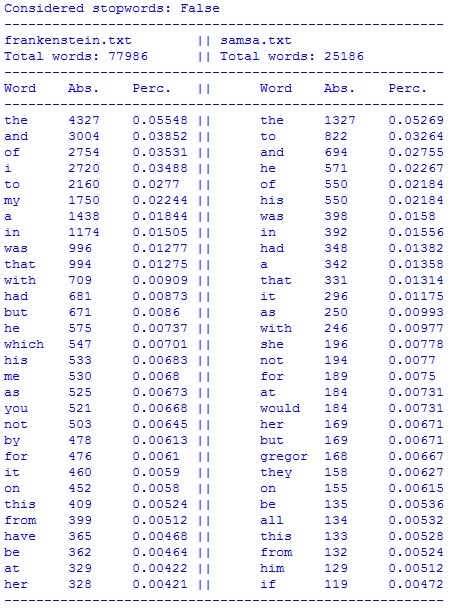
\includegraphics{img/false}
\caption{Liste der 30 am häufigsten vorkommenden Wörter in Frankenstein und Die Verwandlung}
\label{nostopwords}
\end{center}
\end{figure}
Die Einbeziehung einer Liste mit Stopwords soll genau solche Fälle verhindern. In einer solchen Liste sind Wörter enthalten, die keinerlei Aussagekraft über den Inhalt des Textes liefern und deshalb bei der Analyse außen vor gelassen werden sollen. Unter Nichtbeachtung dieser Wörter stellen sich die 30 häufigsten Wörter beider Texte wie in Abb. \ref{stopwords} dar.\\
\begin{figure}[h]
\begin{center}
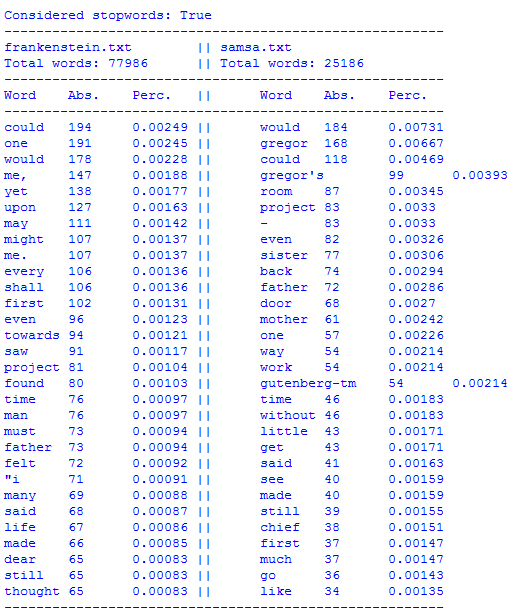
\includegraphics{img/true}
\caption{Liste der 30 am häufigsten vorkommenden Wörter in Frankenstein und Die Verwandlung unter Nichtbeachtung von Stopwords}
\label{stopwords}
\end{center}
\end{figure}
Nun befinden sich unter den 30 Wörtern auch solche, die zumindest grob Rückschlüsse auf den Inhalt der Texte zulassen, wie z. B. \textit{saw}, \textit{time}, \textit{father} (Frankenstein) oder \textit{gregor}, \textit{room}, \textit{sister} (Die Verwandlung).


}
\section*{Aufgabe 3}
\aufgabenstellung{Die Auftrittswahrschein­lichkeit­en von Worten in Tex­ten 
fol­gen einer 
so­ge­nan­nten Zipf-Verteilung, d. h. einer Verteilung, die dop­pelt 
log­a­rith­misch ist. Überprüfen Sie das an­hand der gewählten Texte. (2 
Punk­te) \\
Plot­ten Sie die Häufigkeit­en (y-Achse) über den Rang (x-Achse), also die 
An­zahl der Vorkomm­nisse des häufig­sten Wortes zuerst, dann die An­zahl des 
zwei­thäufig­sten Wortes, etc. Betra­cht­en Sie sowohl eine ab­so­lute als auch 
eine log­a­rith­mis­che Skalierung bei­der Achsen. Was können Sie beobacht­en?\\
Bes­tim­men Sie die An­zahl der Worte, die mit einer gegebe­nen Häufigkeit 
vorkom­men (also, wie viele Wörter gibt es, die mit Häufigkeit 1 vorkom­men, 
wie viele mit Häufigkeit 2, etc. ). Pro­duzieren Sie ähn­liche Grafiken 
(An­zahl der Worte mit einer gewis­sen Häufigkeit über die Häufigkeit) und 
in­ter­pretieren Sie diese.}
\newcommand{\plotOf}[3]{
\begin{figure}[ht]
\begin{center}\resizebox {\columnwidth} {!} {
\begin{tikzpicture}
\begin{axis}
\addplot table [x=i, y=count,col sep=semicolon]
%,col sep=semicolon
{#1};
\end{axis}
\end{tikzpicture}}
\caption{#2}
\label{#3}
\end{center}
\end{figure}
}
\newcommand{\logPlotOf}[3]{
\begin{figure}[ht]
\begin{center}\resizebox {\columnwidth} {!} {
\begin{tikzpicture}
\begin{semilogyaxis}
%[restrict expr to domain={y}{10:1e4},unbounded coords=discard]
\addplot table [x=i, y=count,col sep=semicolon] {#1}; %
\end{semilogyaxis}
\end{tikzpicture}}
\caption{#2}
\label{#3}
\end{center}
\end{figure}
}
\loesung{}
Die Zipf-Verteilung beschreibt, dass die Auftrittswahrscheinlichkeit eines 
Elementes umgekehrt proportional von seiner Position $n$ in einer absteigend 
nach Häufigkeit geordneten Liste von $N$ Elementen
abhängt:\footnote{\url{https://de.wikipedia.org/wiki/Zipfsches_Gesetz}} 
$$p(n) = \frac{1}{H_N} \cdot \frac{1}{n}$$
mit
$$H_N = \sum \frac{1}{n}$$
Inwiefern diese Verteilung Gültigkeit für die Worthäufigkeiten besitzt, wurde 
anhand der Texte aus Aufgabe 2 geprüft. Die Ergebnisse Um die 50 häufigsten 
Wörter samt ihrer 
Häufigkeiten zu ermitteln, wurde unter Verwendung des nltk-Toolkits ein 
Python-Skript\footnote{Zu finden in \tt{aufg03/main.py}} geschrieben, das die 
Daten ermittelt und in eine CSV-Datei schreibt.
Die 
\plotOf{aufg03/frankenstein.txt.csv}{Die Häufigkeit (y-Achse) der 50 
häufigsten Wörter in Frankenstein}{fig:frankensteinHaeufigkeiten} 
\logPlotOf{aufg03/frankenstein.txt.csv}{Die Häufigkeit (y-Achse) der 50 
häufigsten 
Wörter in Frankenstein (logarithmiert)}{fig:frankensteinHaeufigkeitenLog}
\plotOf{aufg03/samsa.txt.csv}{Die Häufigkeit (y-Achse) der 50 häufigsten 
Wörter in Die Verwandlung}{fig:samsaHaeufigkeiten}
\logPlotOf{aufg03/samsa.txt.csv}{Die Häufigkeit (y-Achse) der 50 häufigsten 
Wörter in Die Verwandlung (logarithmiert)}{fig:samsaHaeufigkeitenLog}
\hfill \\
%\csvautotabular
%{aufg03/frankenstein.txt.csv}
\newpage

\begin{figure}[ht]
\begin{center}
\csvreader[
	tabular=|l|l|l|l|l|l|l|,
	head to column names,
	table head=\hline n & Wort & $A\equiv\text{Anzahl}$ & $1/n$ & 
$p(n)\equiv1/(n H_N)$ & $E\equiv p(n) N$ & $1-E/A$ \\ \hline,
	late after line=\\\hline,
	separator=semicolon]{aufg03/frankenstein.txt.csv}{
			i=\i,
			word=\word,
			anzahl=\anzahl,
			rangRatio=\rangRatio,
			p=\p,
			pSumCount=\pSumCount,
			Abw=\Abw
		}
		{
			\i &
			\word &
			\anzahl &
			\rangRatio &
			\p &
			\pSumCount &
			\Abw
		}
\caption{Untersuchung der Gültigkeit des Zipfschen Gesetzes für den Text 
"`Frankenstein"'}
\label{tab:zipfFrankenstein}
\end{center}
\end{figure}

\begin{figure}[ht]
\begin{center}
\csvreader[
	tabular=|l|l|l|l|l|l|l|,
	head to column names,
	table head=\hline n & Wort & $A\equiv\text{Anzahl}$ & $1/n$ & 
$p(n)\equiv1/(n H_N)$ & $E\equiv p(n) N$ & $1-E/A$ \\ \hline,
	late after line=\\\hline,
	separator=semicolon]{aufg03/samsa.txt.csv}{
			i=\i,
			word=\word,
			anzahl=\anzahl,
			rangRatio=\rangRatio,
			p=\p,
			pSumCount=\pSumCount,
			Abw=\Abw
		}
		{
			\i &
			\word &
			\anzahl &
			\rangRatio &
			\p &
			\pSumCount &
			\Abw
		}
\caption{Untersuchung der Gültigkeit des Zipfschen Gesetzes für den Text 
"`Die Verwandlung"'}
\label{tab:zipfVerwandlung}
\end{center}
\end{figure}


	%\rangRatio & 
	%\p & } 
	%\pSumCount & 
	%\theAbw}%


\section*{Aufgabe 4}
Mod­i­fizieren Sie das Pro­gramm, so daß es nicht Worte son­dern a) Buch­staben 
bzw.​ b) Buch­staben­paare zählt.​ Vergle­ichen Sie deren Häufigkeitsverteilung 
sowohl zweier in der gle­ichen Sprache ver­fassten Texte als auch zweier in 
ver­schiede­nen Sprachen abge­fasster Texte.​ (2 Punk­te)
\end{document}
